\newpage
\section{Model Synchronization}
\hypertarget{sec:synch}
\genHeader

At this stage, you have successfully created a trio of rules that can transform a \texttt{Box} with any number of \texttt{Partitions} and
\texttt{Cards} into a \texttt{Dictionary} with an unlimited number of \texttt{Entrys} (or vice versa). Your source and target metamodels are complete, and given
that you probably won't make any further changes to your rules, your correspondence metamodel is also complete.

Now suppose you wanted to make a minor change to one of your current instances, such as adding a single a new card or entry into one of your instances. Could
you modify the instance models and simply run the transformation again to keep the target and sources consistent? 

The current \texttt{fwd.src.xmi} file (Fig.~\ref{fig:ea_extended_fwd_src_xmi}) has a partition with an index of three which, when transformed, correctly
produces a target dictionary with all four entries. What would happen if we attempted to transform this dictionary back into the same learning box, with all
four partitions?

\begin{itemize}

\item[$\blacktriangleright$] Copy and paste \texttt{fwd.trg.xmi}, renaming it as \texttt{bwd.src.xmi}.\footnote{Feel free to either delete or
rename the original \texttt{bwd.src.xmi} for later reference}

\item[$\blacktriangleright$] Run \texttt{LearningBoxToDictionaryIntegrationTrafo.java} and inspect the resulting \texttt{bwd.trg.xmi}
(Fig.~\ref{eclipse:missingP3}). Unforunately, the newest \texttt{part\-it\-ion\-3} is missing!

\vspace{0.5cm}

\begin{figure}[htbp]
\begin{center}
  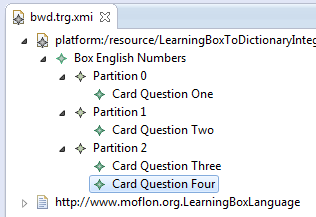
\includegraphics[width=0.5\textwidth]{eclipse_missingPartition}
  \caption{The transformation loses data for any index greater than 2}
  \label{eclipse:missingP3}
\end{center}
\end{figure}
\end{itemize}

As expected, this extra partition was lost because our TGG rules are only able to create exactly three partitions, not additional ones with unique indexing.
How can we prevent data loss when we need to update our models in the future? Luckily, eMoflon can take care of this for you as it provides synchronization
support to update your files incrementally. Let's change our source model by adding a new \texttt{Card} to \texttt{Partition3} and see if the partition still
exists after synchronizing to and from the resulting \texttt{Dictionary} model.

\begin{itemize}

\item[$\blacktriangleright$] Open \texttt{LearningBoxToDictionaryIntegrationSynch.java}, locate the empty \texttt{syncForward} method, and edit it as
shown in Fig.~\ref{eclipse:synchForward}.

\begin{figure}[htbp]
\begin{center}
\begin{lstlisting}[language=Java,backgroundcolor=\color{white}, keywordstyle={\bfseries\color{purple}}]
public void syncForward(String corr) {
	setChangeSrc(root -> { 
		Box box = (Box) root;
		Partition partition3 = box.getContainedPartition()
			.stream().filter(p -> p.getIndex() > 2).findAny().get();
		Card newCard = LearningBoxLanguageFactory.eINSTANCE.createCard();
		newCard.setBack("Question Five");
		newCard.setFace("Answer Fuenf");
		partition3.getCard().add(newCard);
	});
	loadTriple(corr);
	loadSynchronizationProtocol("instances/fwd.protocol.xmi");
	integrateForward();
	saveResult("fwd");
	
	System.out.println("Completed forward synchronization");
}
\end{lstlisting}
  \caption{Implementation of our custom \texttt{IndexToLevel} constraint}
  \label{eclipse:synchForward}
\end{center}
\end{figure}


\item[$\blacktriangleright$] Save and run the file. You'll notice that even though no changes were specified for the backward synchronization, both directions
completed without error.

\item[$\blacktriangleright$] View the results of your changes by first opening your learning box in \texttt{sync.fwd.src.xmi}. Expand \texttt{Partition 3} --
is there now a fifth \texttt{Card} inside? As you can see, the synchronization saved your changes to this new file, rather than overwriting the original
instance model.

\item[$\blacktriangleright$] Open the synchronization's output file, \texttt{sync.bwd.src.xmi}. If it was successful there should be a fifth \texttt{Entry} in
the Dictionary. Together with \texttt{sync.fwd.corr.xmi} and \texttt{sync.fwd.protocol.xmi}, this files form a new triple and will remain consistent with one
another!

\item[$\blacktriangleright$] What if we wanted to make a change in the other direction? Let's try deleting an entry while keeping all four partitions. Open
the synchronization's Java file again and locate \texttt{syncBackward}. Replace the code as depicted in Fig.~\ref{eclipse:synchBacward}.

\newpage

\begin{figure}[htbp]
\begin{center}
\begin{lstlisting}[language=Java,backgroundcolor=\color{white}, keywordstyle={\bfseries\color{purple}}]
public void syncBackward(String corr) {
	setChangeTrg(root -> {
		Dictionary dictionary = (Dictionary) root;
		Entry deleted = dictionary.getEntry().remove(0);
	});
	loadTriple(corr);
	loadSynchronizationProtocol("instances/fwd.protocol.xmi");
	integrateBackward();
	saveResult("bwd");

	System.out.println("Completed backward synchronization");
}
\end{lstlisting}
  \caption{Implementation of our custom \texttt{IndexToLevel} constraint}
  \label{eclipse:synchBacward}
\end{center}
\end{figure}

\item[$\blacktriangleright$] Run the synchronization a final time, and refresh the ``instances'' folder. Open and inspect both \texttt{sync.bwd.src.xmi} and
\texttt{sync.\-bwd.\-trg.\-xmi}. If everything has executed correctly, a \texttt{Card} should be missing in \texttt{Box}, and
\texttt{partition3} still exists! Equivalently, there should only be four \texttt{Entry} elements in the output \texttt{Dict\-ion\-ar\-y}.

\item[$\blacktriangleright$] You may have noticed that there is no \texttt{Entry Five}, which we added to \texttt{partition3} in the forward
synchronization. Recall that the process loads and makes changes to the \emph{original} triple, not the most recent copies. The files are simple Java code, so
you are invited to modify them as you wish for your own projects.

\end{itemize}
